\section{Instantaneous Energetic Cost}
The instantaneous energetic cost, which Bayesian Optimization aims to minimize, is estimated through continuous breath measurements over a lengthy duration of time. \citet{Brockway1987} developed a formula for converting $CO_2$ and $O_2$ measurements into a metabolic cost, which is then fit into a first-order dynamical model. Given the noisiness of respiratory measurements, previous studies \citep{Felt2015,Selinger2014} allowed three minutes while subjects reached a steady state before measuring for an additional three minutes to estimate an instantaneous energetic cost. In a previous Bayesian Optimization study \citep{Ding2018}, each iteration used a fixed two minutes of respiratory measurements. 

Rather than requiring a fixed time interval for each evaluation, we aim to ascertain an accurate estimate only for promising parameter settings while stopping early for those that are unlikely to improve upon the best settings found so far. To make that determination, an online estimator for instantaneous energetic cost was developed using the metabolic cost model
\begin{align}
m_t(c_0, c, \tau_0, \tau) = c(1-e^{\frac{-t}{\tau}}) + c_0e^{\frac{-t}{\tau_0}},
\end{align}
where $t$ is the total measurement time in seconds and $\tau_0, \tau$ are time constants characterizing the rate of change for cost constants $c_0, c$ respectively.

\begin{figure}[t]
\centering
\includegraphics[width=\textwidth]{metabolicestimation.png}
\caption{Sample estimation process for instantaneous energetic cost.}
\label{fig:metabolicestimation}
\end{figure}

\section{Parameter Estimation}
We apply the time and cost constants, including $c$ which represents the instantaneous energetic cost, through an Unscented Kalman Filter \citep{julier1997}. Kalman filters are applied to discrete time systems of the form
\begin{align}\begin{split}
  x(t+1) &= F(x(t), v(t), t)\\
  z(t) &= H(x(t), w(t), t),
\end{split}\end{align}
where $x(t)$ represents the unobserved state of the system, $z(t)$ the observed measurement, and zero-mean Gaussian vectors $v(t)$ for process disturbances or modeling errors and $w(t)$ for measurement noise. 

First, a prediction is made for the state of the system after one timestep. Let $\hat{x}(t\vert t-1)$ represent the estimate for $x(t)$ using measurements $\mathbb{Z}(t-1)=[z(1), z(2), ..., z(t-1)]$ and $P_{x}(t\vert t-1)$ the covariance for the estimate. The prediction step aims to calculate
\begin{align}\begin{split}
  \hat{x}(t\vert t-1) &= \mathbb{E}[F(x(t-1), v(t-1), t-1)\vert \mathbb{Z}(t-1)]\\
  P_{x}(t\vert t-1) &= \mathbb{E}[\{ \hat{x}(t\vert t-1) - x(t) \} \{ \hat{x}(t\vert t-1) - x(t) \}^T \vert \mathbb{Z}(t-1)]
\end{split}\end{align}

The prediction is then reconciled with the observed measurement through a minimum mean-squared estimate $\hat{x}(t)$ and covariance $P_{x}(t)$ according to the following equations
\begin{align}
\begin{split}
  \hat{x}(t) &= \hat{x}(t\vert t-1) + K \mathbb{E}[y] \\
  P_{x}(t) &= P_{x}(t\vert t-1) - KP_{y}(t\vert t-1) K^T\\
  K &= P_{xy}(t\vert t-1) P_{y}^{-1}(t\vert t-1)\\
  y &= z(t) - H(\hat{x}(t\vert t-1) , w(t), t)
\end{split}
\end{align}

The underlying requirement for these equations is an accurate propagation of the first two moments of $x(t)$ and $z(t)$. When $F$ or $H$ is nonlinear, rather than linearizing the functions with a first order approximation the UKF approximates its probability distribution through an unscented transformation. The complete implementation details for the UKF are outlined in Appendix \ref{sec:ukf}.

As we consider $\tau_0, \tau, c, c_0$ to be constant parameters, our UKF setup is
\begin{align}
\begin{split}
  x &= [c \tab c_0 \tab \tau \tab \tau_0]\\
  F(x(t), v(t), t) &= x(t) + v(t)\\
  H(x(t), w(t), t) &= m_t(x(t)) + w(t)
\end{split}
\end{align}

\section{UKF Covariance Parameters}\label{sec:ukfcovar}
The UKF algorithm has covariance parameters $P_{x}$ for the state estimate, $P_{w}$ for measurement noise, and $P_{v}$ for process model noise that determine the sensitivity of the model to new measurements. Table \ref{tab:esttuningparams} summarizes the effect of increasing one of these covariance parameters while holding all others constant.

\begin{figure}[t]
\centering
\includegraphics[width=\textwidth]{measurementnoise.png}
\caption{With a true instantaneous energetic cost at 350 and keeping all other parameters constant, the effect of using $P_w$ variances that are too low, exact, and too high on cost estimate.}
\label{fig:measurementnoise}
\end{figure}

\begin{table}
  \centering
  \begin{tabular}{ | c | p{10cm} |}
  \hline
  Increase In & Effect On State Estimate \\ \hline

  $P_x$ & A higher initial covariance on the state estimate implies higher uncertainty with the state prior. Early observations will have a greater effect on the state update. However, $P_x$ decreases after every state update; observations therefore will have a smaller effect on the state estimate over time\\ \hline

  $P_w$ & A higher measurement noise will reduce an observation's effect on the state update. The state will be to slow to move away from the prior, particularly in early observations\\ \hline

  $P_v$ & While $F$ is essentially the identity function in the metabolics model as the cost and time parameters are assumed to be constant, $P_v$ can be used to enforce a lower bound on the effect of an observation on the state update\\ \hline

  \end{tabular}
  \caption{Tuning Parameters for metabolic estimator}
  \label{tab:esttuningparams}
\end{table}

\section{Subject Testing}
Using previously attained data, Figure \ref{fig:ukftuned} shows the raw and noisy measurements taken and the metabolic cost prediction that the model developed in response to a representative participant\footnote{Testing carried out by Myunghee Kim}. The bottom plot displays the covariance associated with the cost, beginning with a covariance of 1 and converging at different rates depending upon the raw data. When tuned properly, both trials see a relatively smooth rate of convergence of the estimate. With varying amounts of data provided, the accuracy in percent error was calculated by comparing with a "ground truth" value at each termination condition (5 min, 2 min, 1.5 min, 20 breaths, and 30 breaths). This ground truth value is the average of the last two minutes of data, when the subject has reached steady-state.

During the optimization studies, the UKF Estimator showed noisier estimates across various subjects (Figure \ref{fig:subjcostest}). Future work on the estimator would involve creating a cost function to optimize across the various covariance matrices, as these values should also be subject-specific. The cost function should balance between the smoothness of the estimation curve and eventual convergence to the "true cost". The next chapter will go into details on modeling the stopping problem, i.e. how to determine when to stop measuring for a given parameter setting, including how the model changes according to the volatility of the UKF estimator. 

\begin{figure}[t]
\centering
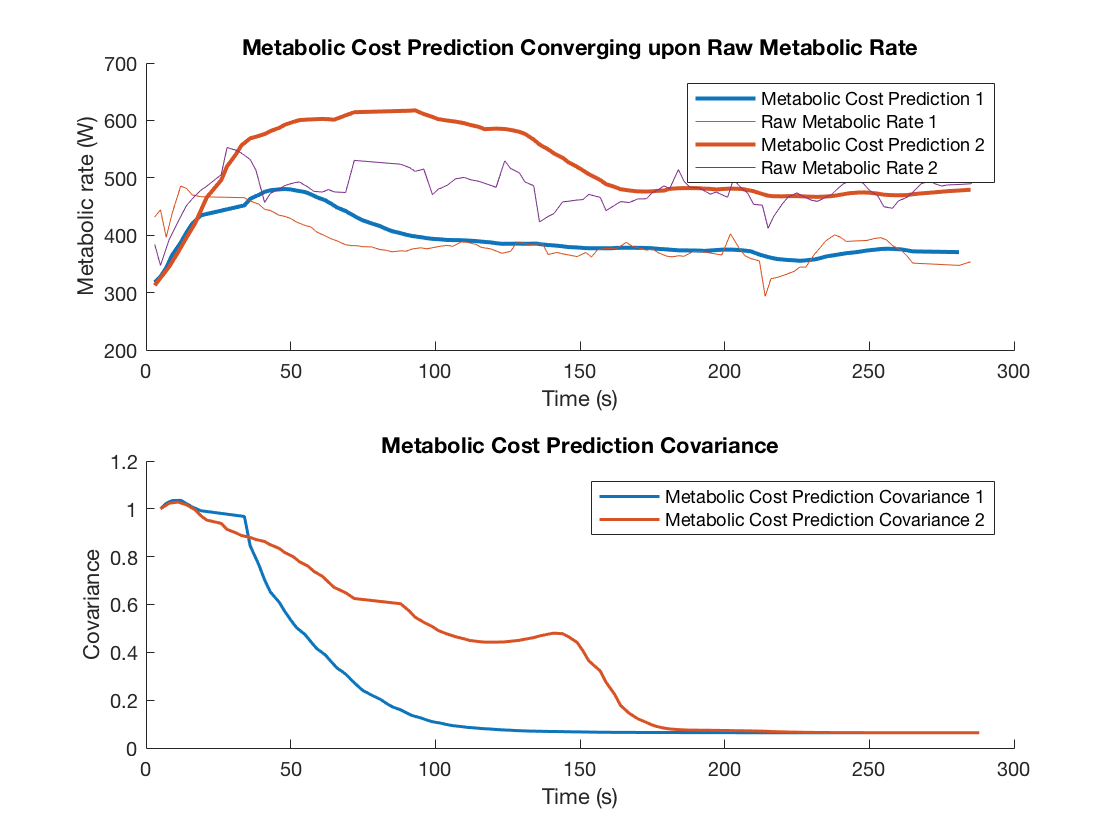
\includegraphics[width=\textwidth]{ukf}

\begin{tabular}{ |c|c|c| } 
 \hline
 Data Used & Average $R^2$ & Max \% Error \\ 
 \hline
 Full Trial & 0.996 & 0.977\% \\ 
 2 Minutes & 0.984 & 0.984\% \\ 
 1.5 Minutes & 0.973 & 0.973\% \\ 
 30 Breaths & 0.966 & 3.113\% \\ 
 20 Breaths & 0.890 & 5.767\% \\ 
 \hline
\end{tabular}%
%}
\caption{Tuned UKF Estimator over previously collected data. Accuracy assessed over partial data.}
\label{fig:ukftuned}
\end{figure}

\begin{figure}[h]
\centering

\includegraphics[width=\textwidth]{subjcostest.png}
\caption{Tuned UKF Estimator shows different levels of noise during optimization studies on different subjects.}
\label{fig:subjcostest}
\end{figure}